% L22eqv.tex
% $Author$ $Date$

% \section{Small $L=22$ system {\rpo s}}
% \label{sec:L22}
% Predrag created file              jul  9 2006

\PCedit{MOTIVATE! MOTIVATE!}

Here we determine
several \eqva\ and many \rpo s for
KS in a periodic cell of size $L=22$.

An instructive example is offered by the dynamics for $L=22$ studied
here.  For this small periodic cell the empirically observed
``sustained turbulence'' arises from a competition between unstable
wavelength 2- and 3- coherent structures.  Of course, as is true of
most realistic ``chaotic'' flows, we have no rigorous way of
establishing that this turbulence is indeed sustained for all time, or
is merely a very long transient to an attracting periodic state.  For
large system size, as the one shown in \reffig{f:ks_largeL}, it is
hard to imagine scenario under which attractive periodic states
(which, as shown in \refref{FSTks86}, exist) would have significantly
large basins of attraction.

The 2-\eqv\  and the 3-\eqv\  essentially lie in
the 2nd and 3rd Fourier component complex plane, with very
small deformations from higher harmonics.
We refer to wavelength 1-, 2- and 3- unstable \eqva\ as
\EQV{1}, \EQV{2} and \EQV{3},
respectively.
In \reffig{f:ks_largeL}
color indicates the value of $u(x,t)$ in 
the $(x,t)$ space-time plane.

\KS\ system with $L = 22$ periodic on the full space is small but
empirically large enough to exhibit persistent chaos.  $L=22$ is a
sensible choice because in units of mean wavelength the size of this
small system is about 2.5 wavelengths ($\tildeL/\sqrt{2}= 2.4758$),
so the dynamics is a competition between wave numbers 2 and 3.
Because of the strong $k^4$ contraction we expect a small
number of modes to be significant for the dynamics, while the
rest are in the numerical noise. See Figure~6 in
\refref{Christiansen:97}.

The leading Lyapunov exponents of the chaotic attractor are 
0.048, 0, 0, -0.003, -0.189, -0.256, -0.290, ... , which shows that 
the attractor lives essentially on a 4-dimensional manifold with strong
contraction in other dimensions.  The two zero exponents correspond to 
time and space translational symmetries of the KS solutions, so the 
dynamics on the attractor appears to be reducible to a 2-dimensional map.

%% Davidchack and Crofts
% We investigate this system in 16 to 64 complex Fourier modes (32 to
%128-dimensional system of real ODEs) truncation, and recheck the results
%by redoing the calculation with the double number of Fourier modes. %
%observe how many digits change. The \eqv\ points are accurate to at least
%to $10^{-11}$. Since Lapack is also double precision accurate, the
%accuracy of the first few eigenvalues is similar, and certainly in excess
%of 6 significant digits. % All digits stated in tables are significant.
%The accuracy that can be reached is of order of
%$|a(\period{p},d_p) - a_0|
% \approx \epsilon \exp(\Lyap_p \period{p})$,
% where $\epsilon \approx 10^{-17}$ for double precision, $\Lyap_p$ is
%the largest Lyapunov exponent, and $\period{p}$ the period.  With a good
%starting guess, Newton's method typically reaches that accuracy after 2-3
%iterates.

\subsection{\Eqva\ and \reqva}

In addition to the trivial \eqv\ $u=0$ (denoted \EQV{0} from now
on), we find for $L = 22$ three \eqva\ with dominant wavenumber $k$
(denoted \EQV{k}) for $k = 1, 2, 3$.  All {\eqva}, shown in
Fig.~\ref{f:KS22Equil}, are symmetric with respect to the reflection
symmetry \refeq{KSparity}. 
In addition, \EQV{2} and \EQV{3} are symmetric with respect
to translation \refeq{KSshift}, 
by $L/2$ and $L/3$, respectively.

\begin{figure}[t]
\begin{center}
(a)\!\!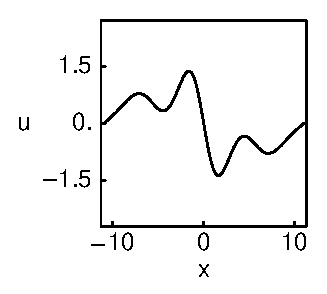
\includegraphics[width=0.27\textwidth]{figs/1wKS22equil.eps}
~~(b)\!\!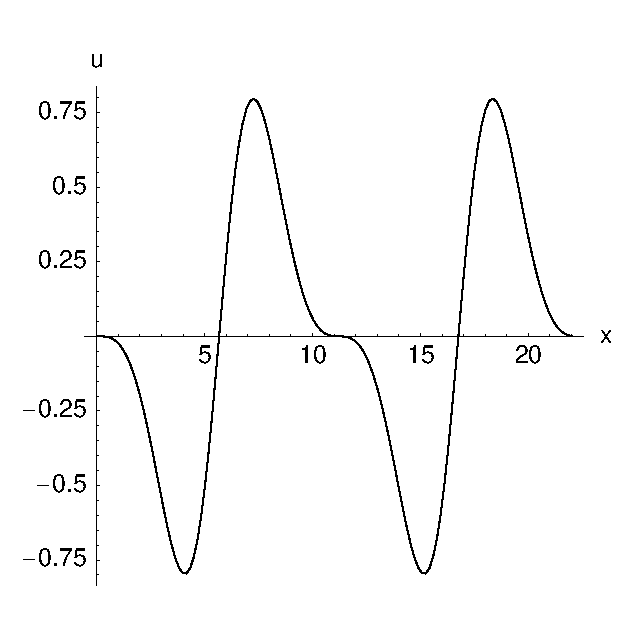
\includegraphics[width=0.27\textwidth]{figs/2wKS22equil.eps}
~~(c)\!\!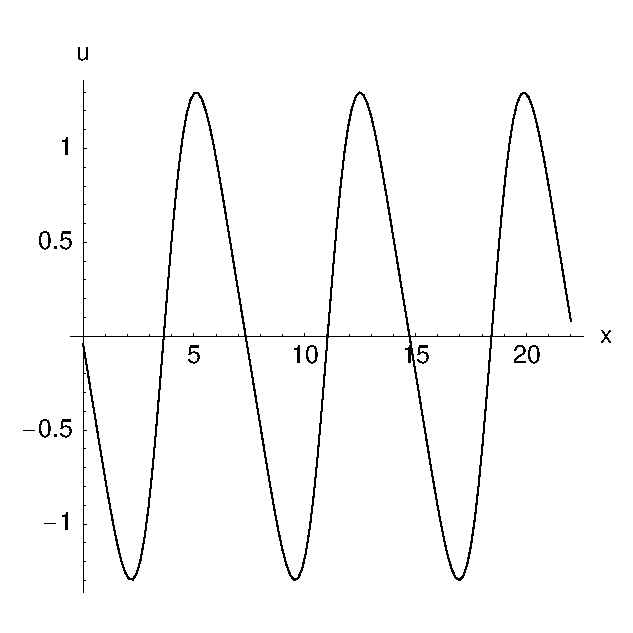
\includegraphics[width=0.27\textwidth]{figs/3wKS22equil.eps}
\end{center}
\caption{ (a) \EQV{1}, (b) \EQV{2}, and (c)
\EQV{3} \eqva. The \EQV{0} \eqv\ is the $u(x)=0$
solution.
$L=22$ system size.
    }
\label{f:KS22Equil}
\end{figure}

The stability of the {\eqva} is characterized by the eigenvalues
$\eigExp[j]$ of the \stabmat.  The leading 10 eigenvalues for each
\eqv\ are listed in \reftab{tab:Eksym}. We compute (available upon request)
the corresponding eigenvectors as well. As an \eqv\ with $\mathrm{Re}
\lambda_j > 0$ is unstable in the direction of the corresponding
eigenvector $\jEigvec{j}$, the eigenvectors provide flow-intrinsic 
(PDE discretization independent) coordinates which we use for visualization
of unstable manifolds and homo- / hetero-clinic connections between
\eqva.

% \begin{table}[t]\label{tab:EkEigs}
% \begin{center} \footnotesize
% \caption{ Eigenvalues of the \eqva\ for $L=22$.}
% \begin{tabular}{cccc} \hline
%   \EQV{0}  &    \EQV{1}        &    \EQV{2}        &  \EQV{3}   \\\hline
%   $0.2198$ &  $0.1308+i0.3341$ &  $0.1390+i0.2384$ &  $0.0933$\\
%   $0.2198$ &  $0.1308-i0.3341$ &  $0.1390-i0.2384$ &  $0.0933$\\
%   $0.1952$ &  $0.0824+i0.3402$ &  $0$              &  $0$\\
%   $0.1952$ &  $0.0824-i0.3402$ & $-0.0840+i0.1602$ & $-0.4128$\\
%   $0.0749$ &  $0$              & $-0.0840-i0.1602$ & $-0.6108+i0.3759$\\
%   $0.0749$ & $-0.2287+i0.1963$ & $-0.1194$         & $-0.6108-i0.3759$\\
%  $-0.3981$ & $-0.2287-i0.1963$ & $-0.2711+i0.3563$ & $-0.6108+i0.3759$\\
%  $-0.3981$ & $-0.2455$         & $-0.2711-i0.3563$ & $-0.6108-i0.3759$\\
%  $-2.1191$ & $-2.0554$         & $-2.0130$         & $-1.6641$\\
%  $-2.1191$ & $-2.0619$         & $-2.0378$         & $-1.6641$\\\hline
% \end{tabular}
% \end{center}
% \end{table}

The eigenvalues of \EQV{0} are determined by the linear part of the KS
equation \refeq{expanMvar}: $\lambda_k=(k/\tilde{L})^2-(k/\tilde{L})^4$.  
For $L=22$, there are three pairs of unstable eigenvalues, corresponding,
in decreasing order, to three unstable modes $k=2,3$, and 1.  For each
mode, the corresponding eigenvectors lie in the plane spanned by
$\Re \, a_k$ and $\Im \, a_k$. \refTab{tab:Eksym}
lists the symmetries of the stability eigenvectors of
\eqva\ \EQV{1} to \EQV{3}.
\PC{
    (a) remove the box within \reffig{f:KS22EkEigs}?  not important...
    (b) Include  \EQV{0} as white circles; we need them, because
    I believe that for larger $k$ all solutions have the same eigenvalues. This
    would enable us to separate dynamical from "hyper-diffusion" spectra,
    tell us how many are dynamically significant. This is different from Navier-Stokes,
    which has zillion contracting complex eigenvalue pairs.
    (c) Make sure the colored points can be distinguished in B\&W. 
   }
% With $S$, $A$ we denote an eigenvector belonging to the symmetric
% or antisymmetric subspace respectively. The last column lists
% the symmetry expected to be present in the corresponding
% stable/ustable manifold.

% \PCedit{I suggest moving \reftab{tab:EkEigs} and related into Appendix,
% replacing them with figures like Gibson's
% \reffig{f:KS22EkEigs}.
%    }

\begin{figure}[t]
\begin{center}
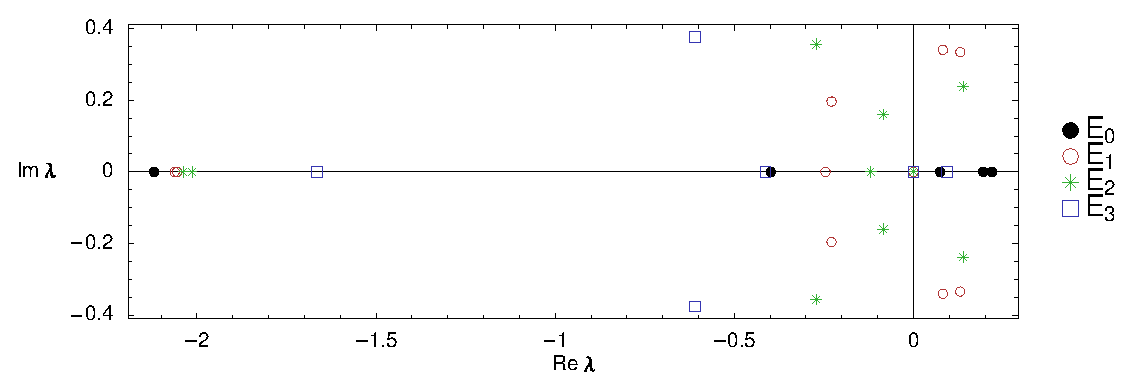
\includegraphics[width=4in]{figs/L22-eqvaEigenvalues.eps}
\end{center}
\caption{
Leading  \eqv\ stability eigenvalues,
$L=22$ system size.
%(b) Eigenvalues of \eqva\ and \reqva\ within
%the symmetric subspace $R_1$.
}
\label{f:KS22EkEigs}
\end{figure}

\begin{table}[t]\label{tab:Eksym}
\caption{
Leading eigenvalues
$\eigExp[j]= \eigRe[j] \pm i\eigIm[j]$
and symmetries of the corresponding eigenvectors
of KS {\eqva} for $L = 22$ system size.
We have used as our reference states the ones that lie on 
the antisymmetric subspace and also listed the symmetries of
the $L/4$ translated ones.
        }
\begin{center} \footnotesize
\begin{tabular}{ccccc} 
\EQV{1}& $\eigRe[j]$ & $\eigIm[j]$ & Symmetry & $A(L/4)\EQV{n}$ Symmetry\\\hline
  $\eigExp[1,2]$ & $0.1308$& $0.3341$ & -  & -\\
  $\eigExp[3,4]$ & $0.0824$& $0.3402$ & $R_1$  & $L$\\
  $\eigExp[5]$   & $0$     &          & -  & -\\
  $\eigExp[6,7]$ &$-0.2287$& $0.1963$ & $R_1$  & $L$\\
  $\eigExp[8]$   &$-0.2455$&          & -  & -\\
  $\eigExp[9]$   &$-2.0554$&          & $R_1$  & $L$\\
  $\eigExp[10]$  &$-2.0619$&          & -  & -\\\hline\\
\EQV{2}&  &  & \\\hline
  $\eigExp[1,2]$ & $0.1390$ & $0.2384$ & $R_1$         & $L$\\
  $\eigExp[3]$   & $0$      &          & $D(2)$        & $D(2)$\\
  $\eigExp[4,5]$ &$-0.0840$ & $0.1602$ & $L$           & $R_1$\\
  $\eigExp[6]$   &$-0.1194$ &          & $D(2)$        & $D(2)$\\
  $\eigExp[7,8]$ &$-0.2711$ & $0.3563$ & $R_1,\,L,\,D(2)$  & $R_1,\,L,\,D(2)$\\
  $\eigExp[9]$   &$-2.0130$ &          & $L$           & $R_1$\\
  $\eigExp[10]$  &$-2.0378$ &          & $R_1$         & $L$\\\hline
\EQV{3}&  &  & \\\hline\\
  $\eigExp[1]$   &$0.0933$  &          & $R_1$     & $L$\\
  $\eigExp[2]$   &$0.0933$  &          & -         & -  \\
  $\eigExp[3]$   &$0$       &          & $D(3)$    & $D(3)$\\
  $\eigExp[4]$   &$-0.4128$ &          & $R_1,\,D(3)$  & $L,\,D(3)$\\
  $\eigExp[5,6]$ &$-0.6108$ & $0.3759$ & $R_1$     & $L$\\
  $\eigExp[7,8]$ &$-0.6108$ & $0.3759$ & -         & -\\
  $\eigExp[9]$   &$-1.6641$ &          & -         & -\\\hline
\end{tabular}
\end{center}
\end{table}


In Fourier coordinates
\(
(\Re a_1, \Im a_1, \Re a_2, \Im a_2, ...)
\,,
\)
 \EQV{2}~\eqv\ has components \(
(0, 0, *, *, 0, 0, *, *,\cdots)
\) - only even modes, while \EQV{3}~{\eqv}
has only $3m$ nonzero modes,
\(
m = 1, 2, 3, \cdots\,,
\)
\ie,
\(
(0,0,0,0,*,*,0,0,0,0,*,*,\cdots)
\,.
\)
They both belong to the antisymmetric subspace, if phases are picked
correctly.
\ie,
you can rotate the phases to make
\( \Re a_k = 0 \)
for all modes. However,
since in addition to
$L$ periodicity, \EQV{k}~{\eqva} have
$L/k$ periodicity, they only have
$kn$ non-zero Fourier modes, the others are identically zero.
% These ``0" are
% really ``0"s, not just small amplitudes.

% \subsection{\Reqva}

In addition to the \eqva, the KS system has pairs of
\reqva\ \refeq{reqva} with fixed profiles
moving at constant speed $\pm c$, \ie,
\PCedit{ $u(x - ct,t)$, so they travel to the right for $c>0$ }
\[ 
u(x \PCedit{-} ct,t) = u(x, 0)\,.
% \quad t \in \mathbb{R}\,.
\]

%%%%%%%%%%%%%%%%%%%%%%%%%%%%%%%%%%%%%%%%%%%%%%%%%%%%%%%%%%%%%%%%%%
\begin{figure}[t]
\begin{center}
\includegraphics[width=0.3\textwidth]{figs/ks22_TW1_profile.eps}
\includegraphics[width=0.3\textwidth]{figs/ks22_TW2_profile.eps}\\
\includegraphics[width=0.3\textwidth]{figs/ks22_TW1_orbit.eps}
\includegraphics[width=0.3\textwidth]{figs/ks22_TW2_orbit.eps}
\end{center}
\caption{
% (a) \Reqv\ \REQV{+}{1}.
% with $L = 22$.
% (b) \Reqv\  \REQV{+}{2}.  
\Reqva : \REQV{+}{1} with velocity $c = 0.737$ and \REQV{+}{2} with
velocity $c = 0.350$.
\REQV{+}{2} belongs to the bifurcation branch starting
at point $M$ in \PCedit{\reffig{fig:ksBifDiag}}.
The upper panels show the \reqva\ profiles.  The lower panels show 
evolution of slightly perturbed \reqva\ and their decay into generic 
turbulence. Each \reqv\ has a reflection symmetric partner related by 
$u(x) \to -u(-x)$ travelling with velocity $-c$.
% , $c \to -c$.
} \label{f:ks22TW}
\end{figure}
%%%%%%%%%%%%%%%%%%%%%%%%%%%%%%%%%%%%%%%%%%%%%%%%%%%%%%%%%%%%%%%%%%

%\PC{ \refeq{f:ks22TW} top panel: remove velocity labels. }
%\PC{split ks22\_RE1-2.eps into four, 
%    so \reffig{f:ks22TW} can be reformatted}
Consistent with the bifurcation diagram of 
Greene and Kim\rf{ksgreene88},
we find two \reqva\ with velocities $c \approx 0.737$ and $0.350$
(labeled \REQV{\pm}{1} and \REQV{\pm}{2},
for ``traveling waves'', from now on).
The profiles of the two \reqva\ and their time evolution
with eventual fall into the chaotic attractor are
shown in \reffig{f:ks22TW}.  The leading eigenvalues of
\REQV{\pm}{1} and \REQV{\pm}{2} are listed in \reftab{tab:TW}.
The eigenvectors do not belong to any of the symmetric 
subspaces of {\KSe} discussed in \refsect{sec:KSeSymm}.
%\PC{please list $c$ in \reftab{tab:TW} }
\begin{table} \label{tab:TW} 
\caption{
Stability eigenvalues of the \reqva\ for $L=22$.
} %\ for $L=22$.}
\begin{center} \footnotesize
\begin{tabular}{ccc|ccc} 
  \multicolumn{3}{c}{\REQV{\pm}{1} ~($c = \pm 0.73699$)}  & 
  \multicolumn{3}{c}{\REQV{\pm}{2} ~($c = \pm 0.34954$)} \\\hline
  &$\eigRe[j]$ & $\eigIm[j]$ & & $\eigRe[j]$ & $\eigIm[j]$\\
  $\eigExp[1,2]$ & $0.1156$ & $0.8173$ & $\eigExp[1]  $ & $0.3370$ & \\
  $\eigExp[3,4]$ & $0.0337$ & $0.4189$ & $\eigExp[2]  $ & $0$ & \\
  $\eigExp[5]$   & $0$      &          & $\eigExp[3,4]$ &$-0.0096$ & $0.6288$\\
  $\eigExp[6]$   &$-0.2457$ &          & $\eigExp[5,6]$ &$-0.2619$ & $0.5591$\\
  $\eigExp[7,8]$ &$-0.3213$ & $0.9813$ & $\eigExp[7,8]$ &$-0.3067$ & $0.0725$\\
\end{tabular}
\end{center}
\end{table}



Plot also the two \eqva\ of \eqva\ points, their
real eigenvectors and their complex eigenplanes. All {\eqva} presumably
wind around these, and as box size $L$ changes, they form continuous
families with smoothly changing $E$. One can check that by
changing $L$ a bit and using the previous \eqv\ to find the next
one.

What does the complex eigenplane continuation does for these
{\eqva} - does it produce nice heteroclinic connections, or is it
wierder? We know there is an analytic formula for a heteroclinic
connection (see \refref{Lan:Thesis}). % Lan's thesis).

The real motivation for all this is that if we understand \eqva\ as
$L \to \infty$ we might have an entry into $L = \infty$ periodic orbit
theory of KS.
\refTab{tab:L22cminus} lists the stability eigenvalues
$\eigExp[1]^-,\eigRe[2]^-\pm\eigIm[2]^-$
of \eqv\ point $E_{-}=(-\sqrt{E},0,0)$
of \refeq{eq:3dks} for $E$ corresponding to each on of \EQV{1}, \EQV{2}
 and \EQV{3} \eqva.
The period of spiraling $T_{-}=2\pi/\theta^-_2$, expansion
rate in the complex plane of spiraling
$\ExpaEig_r\approx\exp(\eigRe[2]^- T_-)$ and contraction
rate along the stable eigendirection
$\ExpaEig_1\approx\exp(\eigRe[1]^- T_-)$ are also listed.

\begin{table}[h!]
    \caption{Who ordered this table? \PCedit{add a digit...}}
\begin{center} \footnotesize
    \begin{tabular}{l|rrrrrr}
                & $E$   &$\eigExp[1]^-$ & $\eigRe[2]^-\pm i \eigIm[2]^-$   & $T$ & $\ExpaEig_r$  & $\ExpaEig_1$  \\ \hline
        $\EQV{1}\ $ &\ 0.13 &\ -0.55    &\ $0.28\pm1.11i$       &\ 5.67     &\ 4.79     &\ 0.04 \\ \hline
        $\EQV{2}\ $     &\ 0.22 &\ -0.66    &\ $0.33\pm1.15i$       &\ 5.47     &\ 5.99     &\ 0.03 \\ \hline
        $\EQV{3}\ $     &\ 0.79 &\ -0.94    &\ $0.47\pm1.29i$       &\ 4.87     &\ 9.92     &\ 0.01
    \end{tabular}
\end{center}
\label{tab:L22cminus}
\end{table}


\subsection{Unstable manifolds of \eqva\ and heteroclinic
connections}

In this section we explore the structure of unstable
manifolds of the {\eqva}.  The \EQV{1} \eqv\ has two unstable
planes within which the solutions are spiralling out (\ie, two
pairs of complex conjugate eigenvalues).  The \EQV{2} has one such plane,
while the \EQV{3} has two real positive eigenvalues, so the solutions are
moving radially away from the \eqv\ within the plane spanned
by the corresponding eigenvectors.  Since \EQV{1} has 
a larger unstable
subspace, it is expected to have much less influence on the
long time dynamics compared to \EQV{2} and \EQV{3}.

\begin{figure}[t]
\begin{center}
\includegraphics[width=0.5\textwidth]{figs/ks22_E1_plane1_manifold.eps}
\includegraphics[width=0.35\textwidth]{figs/ks22_E1_plane1_orbits.eps}
\end{center}
\caption{
The left panel shows the unstable
manifold of \eqv\ \EQV{1} starting within the plane
corresponding to the first pair of unstable eigenvalues. The
coordinate axes $v_1$, $v_2$, and $v_3$ are constructed from vectors
$\mathrm{Re}\,\jEigvec{1}$, $\mathrm{Im}\,\jEigvec{1}$, 
and $\mathrm{Re}\,\jEigvec{6}$
by Gram-Schmidt orthogonalization.
The right panel shows spatial representation of two orbits $A$ and $B$.
The change of color from blue to red indicates increasing values of
$u(x)$.}
\label{f:KS22E1man1}
\end{figure}

To construct an invariant manifold containing solutions
corresponding to the pair of unstable complex conjugate eigenvalues,
$\eigExp = \eigRe \pm i\eigIm$,
$\eigRe > 0$, we start with a set of
initial conditions near \eqv\ \EQV{k},
\beq
  a(0) = a_{{\EQV{k}}} + \epsilon\,\exp(\delta)\jEigvec{j}
\,,
\ee{linUnstMan}
where $\delta$ takes the set of values uniformly distributed in the
interval $[0,2\pi\eigRe/\eigIm]$, $\jEigvec{j}$ is a unit vector in the
unstable plane, and $\epsilon > 0$ is small.

\begin{figure}[t]
\begin{center}
\includegraphics[width=0.48\textwidth]{figs/ks22_E1_plane2_manifold.eps}
\includegraphics[width=0.48\textwidth]{figs/ks22_E1_plane2_orbits.eps}
\end{center}
\caption{
The left panel shows the unstable
manifold of \eqv\ \EQV{1} starting within the plane
corresponding to the second pair on unstable eigenvalues. The
coordinate axes $v_1$, $v_2$, and $v_3$ are constructed from vectors
Re $\jEigvec{3}$, Im $\jEigvec{3}$, and Re $\jEigvec{6}$ 
by Gram-Schmidt orthogonalization.
The right panel shows spatial representation of three orbits. Orbits
$B$ and $C$ pass close to the \eqv\ \EQV{3}.
   }
\label{f:KS22E1man2}
\end{figure}

The manifold starting within the first unstable plane of \EQV{1}, with
eigenvalues $0.1308\pm i\, 0.3341$, is shown in
\reffig{f:KS22E1man1}. It appears to fall directly into the
chaotic attractor.  The behavior of the manifold starting within
the second unstable plane of \EQV{1}, eigenvalues $0.0824\pm i \, 0.3402$, is
remarkably different: as can be seen in \reffig{f:KS22E1man2},
all orbits within the manifold converge to the \eqv\ \EQV{2}.  The
manifold also contains a heteroclinic connection from \EQV{1} to \EQV{3},
and is bordered by the $\eigExp[1]$ unstable manifold of \EQV{3}.
\PC{explain how this is due to symmetry}

\begin{figure}[h]
\begin{center}
\includegraphics[width=0.48\textwidth]{figs/ks22_E2_manifold.eps}%
\includegraphics[width=0.48\textwidth]{figs/ks22_E2_orbits.eps}
\end{center}
\caption{
The left panel shows the two-dimensional
unstable manifold of \eqv\ \EQV{2}. The coordinate axes
$v_1$, $v_2$, and $v_3$ are constructed from vectors
Re $\jEigvec{1}$, Im $\jEigvec{1}$, and $\jEigvec{7}$ by Gram-Schmidt orthogonalization.
The right panel shows spatial representation of three orbits. Orbits
$B$ and $C$ pass close to the \eqv\ \EQV{3}. See 
\reffig{f:KS22Manifold} for a different visualization.
       }
\label{f:KS22E2man}
\end{figure}


%%%%%%%%%%%%%%%%%%%%%%%%%%%%%%%%%%%%%%%%%%%%%%%%%%%%%%%%%%%%%%%%
\begin{figure}[t]
\begin{center} 
%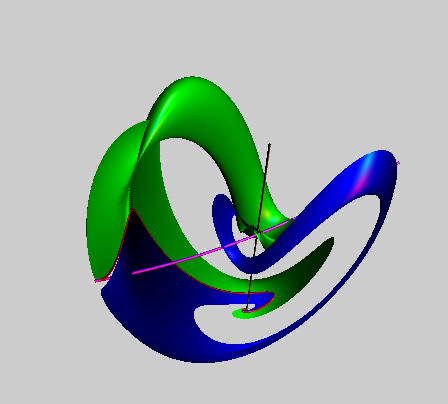
\includegraphics[width=0.6\textwidth]{figs/ks22manifold.ps}
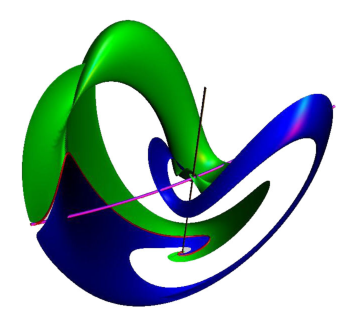
\includegraphics[height=2in]{figs/ks22manifold1.eps}
\end{center}
\caption{
    (blue/green) The unstable manifold of \EQV{2}~\eqv.
%\ of KS equation for $\tilde{L}=3.5014$, N=64 mode truncation.
    (black line) The circle of \EQV{2}~\eqva\ 
related by the translation invariance. 
(purple line) The circle  of \EQV{3}~\eqva.
(red) The heteroclinic connection 
from the \EQV{2}~\eqv\ to the \EQV{3}~\eqv\ splits 
the manifold into two parts, 
colored (blue) and (green).  See 
\reffig{f:KS22E2man} for a different visualization.
        }
\label{f:KS22Manifold}
\end{figure}
%%%%%%%%%%%%%%%%%%%%%%%%%%%%%%%%%%%%%%%%%%%%%%%%%%%%%%%%%%%%%%%%%%

The two-dimensional unstable manifold of \EQV{2} is shown in
\reffig{f:KS22E2man}.  All orbits within the manifold converge
to \EQV{2} shifted by $L/4$.  So this manifold can be viewed as a homoclinic
connection.  It also contains a pair of heteroclinic connections from
\EQV{2} to \EQV{3}.

The \eqv\ \EQV{3} has a pair of real unstable eigenvalues
equal to each other.  Therefore, within the plane spanned by the
corresponding eigenvectors, the orbits move radially away from
the \eqv.  In order to trace out the unstable manifold,
we start with a set of initial conditions within the unstable plane
\beq
 a(0) = a_{{\EQV{3}}} + \epsilon(v_1 \cos \phi + v_2 \sin \phi)\,,
  \quad\phi\in[0,2\pi]\,, 
\label{unsManSeed}
\eeq
where $v_1$ and $v_2$ are orthonormal vectors within the
plane spanned by the two unstable eigenvectors, seeded as in
\refeq{linUnstMan}.
  The unstable manifold
of \EQV{3} is shown in \reffig{f:KS22E3man}.  The 3-fold symmetry of
the manifold is related to the symmetry of \EQV{3} with respect to
translation by $L/3$.  The manifold contains heteroclinic orbits
connecting \EQV{3} to three different points of the continuum of {\eqva}
\EQV{2}
translated by 0 and $\pm L/6$.  Note that there are two different
heteroclinic orbits ($B$ and $C$) connecting \EQV{3} to the same point in the
\EQV{2} continuum.  Note also that the segments of orbits $B$ and $C$
between \EQV{3} and \EQV{2} in \reffigs{f:KS22E1man2}{f:KS22E2man}
represent the same heteroclinic connections as orbits $B$ and $C$ in
\reffig{f:KS22E3man}.

\begin{figure}[t]
\begin{center}
\includegraphics[width=0.45\textwidth]{figs/ks22_E3_manifold.eps}
\includegraphics[width=0.5\textwidth]{figs/ks22_E3_orbits.eps}
\end{center}
\caption{
The left panel shows the two-dimensional
unstable manifold of \eqv\ \EQV{3}. The coordinate axes
$v_1$, $v_2$, and $v_3$ are constructed from vectors
$\jEigvec{1}$, $\jEigvec{2}$, and $\jEigvec{4}$ by Gram-Schmidt orthogonalization.
The black line shows a family of \EQV{2}~\eqva\ related by translational
symmetry. The right panel shows spatial representation of
three orbits. Orbits $B$ and $C$ are two different heteroclinic orbits
connecting \EQV{3} to the same point on the \EQV{2} line.
        }
\label{f:KS22E3man}
\end{figure}

The unstable manifold is traced out in
\reffig{f:KS22E2man1}(a). Computed the 2 expanding eigenvectors
of the \eqv~\EQV{2}, as well as the 3rd, least contracting
direction; then translated and rotated Fourier modes into this
coordinate frame, plotted the unstable manifold.

 It is the unstable manifold of the \EQV{2}
{\eqv}, drawn by tracing out a set of points along one of the complex
eigenvectors, that start close to it. Surprisingly, everybody connects
to the \EQV{2} shifts by 1/2 wavelength ($d = L/4$) but as we are in
$\infty$-dimensions they do it not as the usual homoclinic connection, but in
many (all?) possible intermediate ways. This might be a clue for how to
partition symbolic dynamics.
What is great about
this is that the \EQV{2} unstable manifold has a heteroclinic connection to itself
$L/2$ shifted, but
even better, to \EQV{2}, and \EQV{3} unstable manifold has a heteroclinic
connection to \EQV{2}.
% It's really pretty. 
That makes for a rigid backbone -
we hope this will help us develop a symbolic dynamics for \rpo s.

%Check next what these 2 unstable eigenvectors for \EQV{3}~\eqv\ are - when they
%are equal in magnitude you expect a `star', all directions in their plane
%going straight out. Do they all fall into \EQV{2}~\eqv?

